\documentclass[a4paper,10pt]{report}
\usepackage[utf8]{inputenc}
\usepackage{hyperref}
\usepackage{rotating}
\usepackage{amssymb}
\usepackage{color}


%opening
\title{BRAKER1: Unsupervised RNA-Seq-Based Genome Annotation with GeneMark-ET and AUGUSTUS - \textbf{Supplementary}}
\author{Katharina J. Hoff, Simone Lange, Alexandre Lomsadze,\\ Mark Borodovsky and Mario Stanke}


\begin{document}

\maketitle

\tableofcontents

\chapter{Supplementary Results}



Table \ref{compare} shows  gene prediction accuracy of GeneMark-ET (\textit{ab initio}, first step in BRAKER1) and of AUGUSTUS (trained on GeneMark-ET predictions, using RNA-Seq read alignment information as extrinsic evidence).

\begin{sidewaystable}[h!]
\caption{Accuracy results of GeneMark-ET (\textit{ab initio} predictions) and AUGUSTUS (using RNA-Seq) in BRAKER1 on softmasked genomes.
The AUGUSTUS results are the ones reported for BRAKER1 in Table 1 of the main article. On the fungus \textit{S.~pombe}, GeneMark-ET is superior to AUGUSTUS in the current version of BRAKER1. This is likely to be related to special features in intron splicing mechanism in fungal genomes where the branch point site plays a larger role in splicing than in other species. On the other hand, the acceptor site in fungi plays a smaller role in intron recognition mechanism and carries less signal information. GeneMark-ET has special models to accommodate fungal gene organization, therefore, it delivers accuracy that is difficult to exceed even with use of RNA-Seq information in prediction step. However, in future versions of BRAKER1 with AUGUSTUS adapting such a model we expect to see the same pattern of improving accuracy with respect to pure \textit{ab initio} predictions made by GeneMark-ET. \label{compare}}
\begin{tabular}{lp{1.5cm}p{1.2cm}p{1.5cm}p{1.2cm}p{1.5cm}p{1.2cm}p{1.5cm}p{1.2cm}}\hline
 & \multicolumn{2}{c}{\textit{A.~thaliana}} &  \multicolumn{2}{c}{\textit{C.~elegans}} &  \multicolumn{2}{c}{\textit{D.~melanogaster}} &  \multicolumn{2}{c}{\textit{S.~pombe}}\\
 & \tiny{GeneMark-ET} & \tiny{AUGUSTUS} & \tiny{GeneMark-ET} & \tiny{AUGUSTUS} &  \tiny{GeneMark-ET} & \tiny{AUGUSTUS} & \tiny{GeneMark-ET} &\tiny{AUGUSTUS}\\
 \hline
Gene sensitivity        & 52.6 & \textbf{64.4} & 42.8 & \textbf{55.0} & 54.6 & \textbf{67.6} & \textbf{81.6} & 77.4\\
Gene specificity        & 51.0 & \textbf{52.0} & 42.4 & \textbf{55.2} & 55.1 & \textbf{61.1} & \textbf{84.2} & 80.5\\
Transcript sensitivity  & 44.5 & \textbf{55.0} & 32.7 & \textbf{43.0} & 39.8 & \textbf{50.2} & \textbf{81.6} & 77.4\\
Transcript specificity  & \textbf{51.0} & 50.9 & 42.4 & \textbf{53.2} & 55.1 & \textbf{59.9} & \textbf{84.2} & 76.5\\
Exon sensitivity        & 80.5 & \textbf{82.9} & 79.7 & \textbf{80.2} & 66.6 & \textbf{73.3} & \textbf{87.6} & 83.2\\
Exon specificity        & 77.9 & \textbf{79.0} & 78.7 & \textbf{85.3} & 62.1 & \textbf{67.3} & \textbf{88.4} & 83.2\\
\hline
\end{tabular}
\end{sidewaystable}


Accuracy results of BRAKER1 in unmasked genomes are shown in Table \ref{unmasked}.


\begin{table}[h!]
\caption{Accuracy results of BRAKER1 in unmasked genomes of four model organisms. \label{unmasked}}
\begin{tabular}{lp{.9cm}p{.9cm}p{.9cm}p{.9cm}}\hline
 & \multicolumn{1}{c}{\textit{A.~thaliana}} &  \multicolumn{1}{c}{\textit{C.~elegans}} &  \multicolumn{1}{c}{\textit{D.~melanogaster}} &  \multicolumn{1}{c}{\textit{S.~pombe}}\\
 \hline
Gene sensitivity        & 63.9 & 55.0 & 68.4 & 77.0\\
Gene specificity        & 51.6 & 55.2 & 60.6 & 80.1\\
Transcript sensitivity  & 54.6 & 43.2 & 50.6 & 77.0\\
Transcript specificity  & 50.4 & 53.3 & 59.3 & 76.1\\
Exon sensitivity        & 82.5 & 79.8 & 73.7 & 83.0\\
Exon specificity        & 78.8 & 85.4 & 67.1 & 82.9\\
\hline
\end{tabular}
\end{table}

MAKER2 is an annotation pipeline that automatically repeat masks genomes, executes several gene finders (in our case SNAP, AUGUSTUS and GeneMark-ES), integrates extrinsic evidence when specifies and creates a ``combined gene set'' from all information input sources. We trained SNAP and AUGUSTUS on intermediate MAKER2 results that were generated with Cufflinks assembled RNA-Seq data. GeneMark-ES is a self-training algorithm that requires a genome sequence, only. Table \ref{single_preds_maker} shows \textit{ab initio} prediction results of SNAP, AUGUSTUS and GeneMark-ES applied to unmasked genomes with the parameters that were used for running MAKER2. In comparison to the final MAKER2 results (see Table 1 in the main manuscript), MAKER2 improves gene prediction accuracy by adding RNA-Seq evidence, repeat masking and combining results.

\begin{sidewaystable}[h!]
\caption{\textit{Ab initio} prediction accuracy of SNAP, AUGUSTUS and GeneMark-ES (as trained for running MAKER2) on unmasked genomes. (Transcript specificity is not shown since it is in this case identical to Gene specificity; none of the methods predicted alternative transcripts in \textit{ab initio} mode.) \label{single_preds_maker}}
\begin{tabular}{|l|p{1.5cm}p{1.2cm}p{1.2cm}|p{1.2cm}p{1.2cm}p{1.2cm}|p{1.2cm}p{1.2cm}p{1.2cm}|p{1.2cm}p{1.2cm}p{1.2cm}|}\hline
 & \multicolumn{3}{c}{\textit{A.~thaliana}} &  \multicolumn{3}{|c|}{\textit{C.~elegans}} &  \multicolumn{3}{|c|}{\textit{D.~melanogaster}} &  \multicolumn{3}{|c|}{\textit{S.~pombe}}\\
 & \tiny{SNAP} & \tiny{AUGUSTUS} & \tiny{GeneMark-ES} & \tiny{SNAP} & \tiny{AUGUSTUS} &  \tiny{GeneMark-ES} & \tiny{SNAP} & \tiny{AUGUSTUS} &\tiny{GeneMark-ES} & \tiny{SNAP} & \tiny{AUGUSTUS} & \tiny{GeneMark-ES}\\
 \hline
Gene sensitivity        & 14.5 & 37.5 & \textbf{50.7} & 21.0 & 23.9 & \textbf{42.4} & 40.8 & 41.3 & \textbf{52.6} & 50.3 & 61.8 & \textbf{80.8}\\
Gene specificity        & 11.2 & 32.1 & \textbf{44.3} & 15.3 & 25.7 & \textbf{41.1} & 30.6 & 37.6 & \textbf{50.3} & 49.4 & 67.4 & \textbf{84.2}\\
Transcript sensitivity  & 11.9 & 31.6 & \textbf{42.7} & 16.4 & 18.3 & \textbf{32.3} & 30.4 & 29.6 & \textbf{38.4} & 50.3 & 61.8 & \textbf{80.8}\\
Exon sensitivity        & 58.7 & 71.5 & \textbf{80.3} & 67.9 & 69.1 & \textbf{80.0} & 57.4 & 56.3 & \textbf{66.1} & 66.4 & 64.8 & \textbf{87.6}\\
Exon specificity        & 44.3 & 66.5 & \textbf{68.8} & 53.1 & 72.1 & \textbf{77.2} & 43.5 & 53.2 & \textbf{56.9} & 56.4 & 69.7 & \textbf{88.4}\\
\hline
\end{tabular}
\end{sidewaystable}

In order to demonstrate that parameter training for AUGUSTUS with BRAKER1 works well, we show \textit{ab initio} gene prediction accuracy of AUGUSTUS trained by experts (as distributed via the AUGUSTUS release) and trained by BRAKER1 fully automatically in table \ref{single_preds_braker}.

\begin{sidewaystable}[h!]
\caption{\textit{Ab initio} prediction accuracy of AUGUSTUS trained by experts and fully automatically trained by BRAKER1 on softmasked genomes. (Transcript specificity is not shown since it is in this case identical to Gene specificity; AUGUSTUS did not predict alternative transcripts in \textit{ab initio} mode.) \label{single_preds_braker}}
\begin{tabular}{lp{1.5cm}p{1.2cm}p{1.2cm}p{1.2cm}p{1.2cm}p{1.2cm}p{1.2cm}p{1.2cm}}\hline
 & \multicolumn{2}{c}{\textit{A.~thaliana}} &  \multicolumn{2}{c}{\textit{C.~elegans}} &  \multicolumn{2}{c}{\textit{D.~melanogaster}} &  \multicolumn{2}{c}{\textit{S.~pombe}}\\
 & \tiny{Expert} & \tiny{BRAKER1} & \tiny{Expert} & \tiny{BRAKER1} &  \tiny{Expert} & \tiny{BRAKER1} & \tiny{Expert} &\tiny{BRAKER1}\\
 \hline
Gene sensitivity        & \textbf{51.8} & 49.2 & \textbf{45.2} & 42.3 & 53.2 & \textbf{56.1} & \textbf{78.4} & 70.5 \\
Gene specificity        & \textbf{56.6} & 48.2 & 43.2 & \textbf{46.2} & \textbf{63.4} & 53.7 & \textbf{84.8} & 76.0  \\
Transcript sensitivity  & \textbf{44.2} & 41.6 & \textbf{35.2} & 32.7 & 39.0 & \textbf{41.1} & \textbf{78.4} & 70.4  \\
Exon sensitivity        & \textbf{79.8} & 76.4 & \textbf{76.1} & 74.9 & \textbf{67.7} & 65.0 & \textbf{84.7} & 73.2  \\
Exon specificity        & \textbf{81.7} & 79.8 & 81.5 & \textbf{83.4} & \textbf{67.4} & 63.3 & \textbf{89.4} & 83.1  \\
\hline
\end{tabular}
\end{sidewaystable}

\chapter{Supplementary Methods}

\begin{figure}[!tpb]%figure1
\centerline{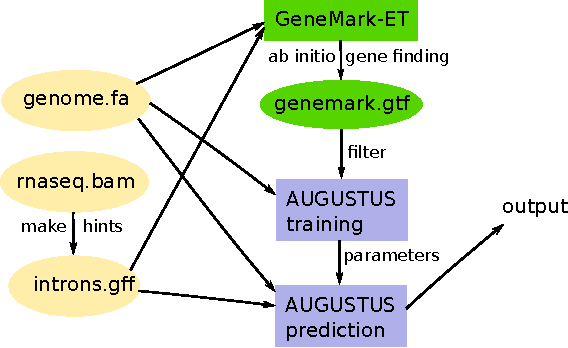
\includegraphics[width=0.7\linewidth]{figs/Figure1.pdf}}
\caption{Schematic view of the BRAKER1 pipeline.}\label{pipeline}
\end{figure}

\section{Test Data}

In order to demonstrate prediction accuracy, nuclear genomes, reference annotations and RNA-Seq libraries were retrieved for four model organisms from the respective databases: for \textit{Arabidopsis thaliana}, TAIR 10 from \url{http://arabidopsis.org}; for \textit{Caenorhabditis elegans}, WS240 from \url{http://www.wormbase.org}; for \textit{Drosophila melanogaster}, R5 from \url{http://flybase.org}; for \textit{Schizosaccharomyces pombe}, ASM294v2.23 from \url{http://www.pombase.org}. The following RNA-Seq libraries were retrieved from the short read archive at NCBI: SRR934391 (for \textit{A.~thaliana}); SRR065719 (for \textit{C.~elegans}); SRR023505, SRR023546, SRR023608, SRR026433, SRR027108 (for \textit{D.~melanogaster}); SRR097898-SRR097900, SRR097902, SRR097903,
SRR097905-SRR097909, SRR097912, SRR097915, SRR097917, SRR097921, SRR097922, SRR097925, SRR402833 (for \textit{S.~pombe}).

\section{RNA-Seq Alignment}

RNA-Seq libraries were aligned against the respective genomes with TopHat2 version 2.0.11 \cite{TopHat2} using Bowtie2 version 2.2.2\\ \cite{Bowtie2}.

In order to determine library specific characteristics such as insert size, TopHat2 was first run with standard parameters. Initial alignments were processed with Cufflinks \cite{Cufflinks} version 2.2.0. The Cufflinks run was interrupted after the output showed ``Fragment Length Distribution'' parameters. Subsequently, TopHat2 was run with the such determined mean insert size and standard deviation. Table \ref{Tab:01} shows Tophat2 parameters that were used for all sets of RNA-Seq libraries in this publication.

\begin{sidewaystable}
\begin{center}
\begin{tiny}
 \begin{tabular}{p{0.2\textwidth} c c c c c c c}
 \hline
Library & \texttt{--mate-inner-dist} & \texttt{--mate-std-dev} & \texttt{--min-intron-length} & \texttt{--min-coverage-intron} & \texttt{--min-segment-intron} & \texttt{--microexon-search} & \texttt{--max-intron-length} \\
\hline
SRR934391 & 20 & 46 & -- &  -- & -- & \checkmark & 100000\\
SRR065719 & 14 & 25 &20&20&20& \checkmark & 100000\\
SRR023505, SRR023546, SRR023608, SRR026433, SRR027108 & 38 & 26 & 30 & 30 & 30 & \checkmark & --\\
SRR097898, SRR097899, SRR097900, SRR097902, SRR097903, SRR097905, SRR097906, SRR097907, SRR097908, SRR097909, SRR097912, SRR097915, SRR097917, SRR097921, SRR097922, SRR097925, SRR402833  & -- & -- & 20 & 20 & 20 & \checkmark & 100000\\
\hline
 \end{tabular}
 \end{tiny}
 \end{center}
\caption{\label{Tab:01}TopHat2 parameters used for RNA-Seq alignment.}
\end{sidewaystable}

\section{Cufflinks Assembly}

MAKER2 \cite{MAKER2} and CodingQuarry \cite{CodingQuarry} require an RNA-Seq assembly. We used Cufflinks version 2.2.0 with standard parameters to assemble the libraries that had previously been aligned to the genome with TopHat2. 

\section{Repeat Masking}

Genomes were softmasked for repeats using RepeatModeler 1.0.8 \cite{RepeatModeler}.

\section{Running BRAKER1}

The command for running BRAKER1 version 1.5 with GeneMark-ET version 4.28 and AUGUSTUS version 3.1.0 on softmasked genomes was\\

\noindent \texttt{braker.pl --genome=genome.fa --species=speciesname --bam=accepted\_hits.bam --softmasked}\\

\noindent where \texttt{accepted\_hits.bam} is the TopHat2 alignment file and \texttt{speciesname} is a name for storing output parameters.

\noindent For unmasked genomes, the command flag \texttt{--softmasked} was removed.

\noindent For \textit{S.~pombe}, BRAKER1 was run with the flag \texttt{--fungus} which enable usage of the fungi-specific branchpoint model of GeneMark-ET.

\section{Running MAKER2}

For running MAKER2, we followed the tutorial at \url{http://weatherby.genetics.utah.edu/MAKER/wiki/index.php/MAKER_Tutorial_for_GMOD_Online_Training_2014}, mostly.

A database of transposable elements and a RepBase repeat library were used for repeat masking with MAKER2.

MAKER2 was run with the gene finders SNAP \cite{SNAP}, AUGUSTUS \cite{AUGUSTUS}, and GeneMark-ES \cite{GeneMark-ES}. MAKER2 was developed to run with protein database to support gene discovery. We did not enable database support because BRAKER1 has no such feature. Thus, MAKER2 - in the way that we used it - is a method that calls and masks repeats, generates training gene structures on the basis of RNA-Seq data, and predicts genes with extrinsic evidence from RNA-Seq data. Running MAKER2 on a novel species consists of three steps: 

\begin{enumerate}
 \item Generating training gene structures for SNAP and AUGUSTUS with MAKER2,
 \item training SNAP, AUGUSTUS and GeneMark-ES (outside of MAKER2), and
 \item predicing genes with MAKER2 using GeneMark-ES, SNAP and AUGUSTUS.
\end{enumerate}

\noindent Training gene structures can be improved an iterative fashion. We computed two iterations.

Training of the gene prediction tool GeneMark-ES depends on the genome sequence, only, and is therefore independent of MAKER2. GeneMark-ES was trained using the command\\

\noindent \texttt{gm\_es.pl genome.fa}

\noindent For \textit{S.~pombe}, GeneMark-ES was trained using the flag \texttt{--fungus} to enable the fungi-specific branch point model in GeneMark-ES.

\subsection{Generating training gene structures for SNAP and AUGUSTUS (first iteration)} \label{training_genes_it1}

MAKER2 configuration files were generated\\

\noindent \texttt{maker -CTL}\\

\noindent The file \texttt{maker\_opts.ctl} was edited to contain (besides default parameters):

\begin{verbatim}
genome=genome.fasta
est=transcripts.fa # Cufflinks assembly
est2genome=1
\end{verbatim}

\noindent No HMMs for gene finders were configured. MAKER2 was run with the following command:\\

\noindent \texttt{maker}\\

\noindent Chromosome-specific \texttt{gff} files were converted to \texttt{ann/zff} and \texttt{dna} files (native format for training SNAP):

\begin{verbatim}
# maker2zff belongs to MAKER2
maker2zff Chr.gff
mv genome.ann genome.Chr.ann
mv genome.dna genome.Chr.dna
cat genome.Chr.ann ... > genome.ann
cat genome.Chr.dna ... > genome.dna
\end{verbatim}

\noindent To obtain a training gene file for AUGUSTUS, \texttt{ann/zff} files were first converted to \texttt{gff3}, and from there to \texttt{gtf}:

\begin{verbatim}
# zff2gff3.pl belongs to SNAP
zff2gff3.pl genome.Chr.ann > Chr.gff3
cat Chr.gff3 | perl -ne '
  if(not(m/^\#/)){
    chomp; @t = split(/\t/); 
    @t2 = split(/=/, $t[7]);
    print "$t[0]\t$t[1]\t$t[2]\t$t[3]\t$t[4]\t$t[5]\t$t[6]\t";
    print "\tgene_id \"$t2[1]Chr\"; transcript_id"; 
    print "  \"$t2[1]Chr\"\n";
  }'> Chr.gtf
# the last two lines makes gene/transcript IDs unique across 
# different chromosomes

# join gtf files from different chromosomes:
cat Chr.gtf ... > all.gtf
\end{verbatim}

\noindent AUGUSTUS training genes are excised with a flanking noncoding region. In BRAKER1, the average gene length divided by two is used as a flanking region length. The average gene length and resulting flanking region length were computed:

\begin{verbatim}
cat all.gtf | perl -ne '
  @t = split(/\t/);
  $seen{$t[8]} += ($t[4] - $t[3] + 1); 
  if(eof()){
    $sum = 0; $c = 0; 
    foreach my $key ( keys %seen ){
    $c=$c+1; $sum += $seen{$key};} 
    print $sum."/".$c."=".($sum/$c); 
    print "\n";
  }'
# the resulting number was divided by two
\end{verbatim}

\noindent This resulted in the following flanking region lengths that were used for excising training genes from the genome for training AUGUSTUS for MAKER2 (first iteration):\\

\begin{center}
\begin{tabular}{l r}
\hline
Species & Flanking region length (nt)\\
\hline
\textit{Arabidopsis thaliana} & 644\\
\textit{Caenorhabditis elegans} & 616\\
\textit{Drosophila melanogaster} & 972\\
\textit{Schizosaccharomyces pombe} & 1050\\
\hline
\end{tabular}
\end{center}

\noindent The \texttt{gtf} file was converted to a \texttt{gb} file with above flanking region length:\\

\begin{verbatim}
# gff2gbSmallDNA.pl belongs to AUGUSTUS
gff2gbSmallDNA.pl all.gtf genome.fasta $flanking_region_length first.gb
\end{verbatim}

\noindent Above described procedure lead to the generation of the following numbers of training genes:

\begin{center}
\begin{tabular}{l r}
\hline
Species & Number of training genes\\
\hline
\textit{Arabidopsis thaliana} & 13547\\
\textit{Caenorhabditis elegans} & 7660\\
\textit{Drosophila melanogaster} & 7049\\
\textit{Schizosaccharomyces pombe} & 307\\
\hline
\end{tabular}
\end{center}

\subsection{Training SNAP and AUGUSTUS (first iteration)}

\subsubsection{Training SNAP} \label{train_snap_it1}

\begin{verbatim}
# fathom, forge and hmm-assembler.pl are part of SNAP
fathom -categorize 1000 genome.ann genome.dna
fathom -export 1000 -plus uni.ann uni.dna
forge export.ann export.dna
hmm-assembler.pl ${species} . > ${species}.hmm
\end{verbatim}

\subsubsection{Training AUGUSTUS} \label{train_augustus_it1}

A new species for AUGUSTUS parameters was created:

\begin{verbatim}
# new_species.pl is part of AUGUSTUS
new_species.pl --species=${species}
\end{verbatim}


\noindent The original training gene structure contained errors, such as occasionally missing start- or stop-codons. Such error containing genes were filtered out:\\

\begin{verbatim}
# etraining and filgerGenesOut_mRNAname.pl are part of AUGUSTUS
etraining --species=maker2_spomb1 first.gb 1> etrain-test.out 
   2> etrain-test.err
   
fgrep "gene" etrain-test.err | cut -f 2 -d " " > bad.etraining-test.lst

filterGenesOut_mRNAname.pl bad.etraining-test.lst first.gb > second.gb

etraining --species=maker2_spomb1 second.gb
\end{verbatim}

\noindent The training gene set was split into two sets, the second set was subsequently further split in another two sets, resulting in three different files:

\begin{enumerate}
 \item A small ``test set'' of 200 (in case of \textit{S.~pombe} first iteration: 23) genes for measuring accuracy after \texttt{etraining} and \texttt{optimize\_augustus.pl}, 
 \item a large gene set for \texttt{etraining}, that was further split into:
 \begin{enumerate}
 \item a large gene set for for the option \texttt{--onlytrain} of \\\texttt{optimize\_augustus.pl},
 \item a small gene set for \texttt{optimize\_augustus.pl}, the size was 1000 for all species except for \texttt{S.~pombe}, where genes were not further split due to their small number.
 \end{enumerate}
\end{enumerate}

\begin{verbatim}
# randomSplit.pl is part of AUGUSTUS
randomSplit.pl second.gb 200
randomSplit.pl second.gb.train 1000
# this results in the following files:
# 1) second.gb.test -> measuring accuracy
# 2) second.gb.train -> etraining
# 2a) second.gb.train.train -> --onlytrain in optimize_augustus.pl
# 2b) second.gb.train.test -> optimize_augustus.pl
\end{verbatim}

\noindent Major AUGUSTUS parameters were ajusted with \texttt{etraining}:\\

\noindent \texttt{etraining --species=\$\{species\} second.gb.train}\\

%\noindent Accuracy after \texttt{etraining} was tested with:\\

%\noindent \texttt{augustus --species=\$\{species\} second.gb.test}\\

%\noindent Accuracy results after different training steps are summarized in table \ref{TrainAcc}.
\noindent Other parameters were optimized with \texttt{optimize\_augustus.pl:}\\

\noindent \texttt{optimize\_augustus.pl --species=\$\{species\} --onlytrain=second.gb.train.train second.gb.train.test}\\

%\noindent Accuracy after \texttt{optimize\_augustus.pl} was tested with:\\

%\noindent \texttt{augustus --species=\$\{species\} second.gb.test}\\

\subsection{Generating training gene structures (second iteration)}

\subsubsection{Generating training gene structures for SNAP}

MAKER2 parameters were generated:\\

\noindent \texttt{maker -CTL}\\

\noindent The file \texttt{maker\_opts.ctl} was edited to contain (besides default parameters):

\begin{verbatim}
genome=genome.fasta
est=transcripts.fa # Cufflinks assembly
snaphmm=${species}.hmm
\end{verbatim}

\noindent MAKER2 was run with the following command:\\

\noindent \texttt{maker}\\

\noindent Training gene extraction for SNAP was performed as described for iteration 1 in section \ref{training_genes_it1}.

\subsubsection{Generating training gene structures for AUGUSTUS}

MAKER2 parameters were generated:\\

\noindent \texttt{maker -CTL}\\

\noindent The file \texttt{maker\_opts.ctl} was edited to contain (besides default parameters):

\begin{verbatim}
genome=genome.fasta
est=transcripts.fa # Cufflinks assembly
augustus_species=${species}
\end{verbatim}

\noindent MAKER2 was run with the following command:\\

\noindent \texttt{maker}\\

\noindent Training gene extraction for AUGUSTUS was performed as described for iteration 1 in section \ref{training_genes_it1}, leading to the following numbers of training genes:

\begin{center}
\begin{tabular}{l r}
\hline
Species & Number of training genes\\
\hline
\textit{Arabidopsis thaliana} & 11887\\
\textit{Caenorhabditis elegans} & 5711\\
\textit{Drosophila melanogaster} & 7568\\
\textit{Schizosaccharomyces pombe} & 1013\\
\hline
\end{tabular}
\end{center}

\subsection{Training SNAP and AUGUSTUS (second iteration)}

\subsubsection{Training SNAP}

Training SNAP was performed as described in section \ref{train_snap_it1}.

\subsubsection{Training AUGUSTUS}

Training AUGUSTUS was performed as described in section \ref{train_augustus_it1}, except that no new species was created (parameters of iteration 1 were refined).

\subsection{Predicting genes with MAKER2}

\subsubsection{Preparing \texttt{rnaseq.gff3}}

Junctions generated by TopHat2 and Cufflinks transcripts were converted to \texttt{gff3} format:

\begin{verbatim}
# tophat2gff3 and cufflinks2gff3 are part of MAKER2
tophat2gff3 junctions.bed > tophat.gff3
cufflinks2gff3 transcripts.gtf > cufflinks.gff3
cat tophat.gff3 cufflinks.gff3 > rnaseq.gff3
\end{verbatim}


\subsubsection{Running MAKER2}

MAKER2 parameters were generated:\\

\noindent \texttt{maker -CTL}\\

\noindent The file \texttt{maker\_opts.ctl} was edited to contain (besides default parameters):

\begin{verbatim}
genome=genome.fasta
est=transcripts.fa # Cufflinks assembly
est_gff=rnaseq.gff3 # TopHat2 and Cufflinks
augustus_species=${species}
snaphmm=${species}.hmm #SNAP HMM file
gmhmm=${species}/gmhmm.mod #GeneMark HMM file
augustus_species=${species} # AUGUSTUS model
keep_preds=1
\end{verbatim}

\noindent MAKER2 was run with the following command:\\

\noindent \texttt{maker}\\

\section{Running CodingQuarry}

As a tool specific for fungi, we ran CodingQuarry on \textit{S.~pombe}, only. First, Cufflinks assemblies were converted from \texttt{gtf} to \texttt{gff3}, then CodingQuarry was executed:

\begin{verbatim}
CufflinksGTF_to_CodingQuarryGFF3.py transcripts.gtf > transcripts.gff3

CodingQuarry -f genome.fasta -t transcripts.gff3 -d -p 8
\end{verbatim}


\section{\textit{Ab initio} Gene Predictions}

In order to show that using RNA-Seq data is beneficial to gene prediction accuracy as compared to \textit{ab initio} prediction, genes were predicted \textit{ab initio} with parameters that were used for running MAKER2 and BRAKER1, respectively.

\subsection{For comparison with MAKER2}

SNAP, AUGUSTUS and GeneMark-ET were used for running MAKER2. \textit{Ab initio} predictions were produced with the following commands:

\begin{verbatim}
snap species_specific_maker2_snap_model unmasked_genome.fa > snap.zff
augustus species=species_specific_maker2_augustus_model unmasked_genome.fa > augustus.out
gmes_petap.pl  --ES  --sequence unmasked_genome.fa --pbs --v
\end{verbatim}

\subsection{For comparison with BRAKER1}

AUGUSTUS was run with \textit{expert trained} parameters as distributed with the AUGUSTUS release (parameter set \texttt{arabidopsis} for \textit{A.~thaliana}, \texttt{caenorhabditis} for \textit{C.~elegans}, \texttt{fly} for \textit{D.~melanogaster} and \texttt{schizosaccharomyces\_pombe} for \textit{S.~pombe} in \textit{ab initio} mode on softmasked genomes with the following command:

\begin{verbatim}
augustus --species=species --softmasking=on softmasked_genome.fa > augustus.out 
\end{verbatim}

\noindent AUGUSTUS was also run in \textit{ab initio} mode using the exact same command with the parameters trained by BRAKER1 for each species.


\section{Measuring Accuracy}

Accuracy was measured using the Eval package \cite{Eval}.



\begin{thebibliography}{}
\bibitem[Kim {\it et~al}., 2013]{TopHat2} Kim, D. and Pertea, G. and Trapnell, C. and Pimentel, H. and Kelley, R. and Salzberg, S.L. (2013) TopHat2: accurate alignment of transcriptomes in the presence of insertions, deletions and gene fusions, {\it Genome Biology} \textbf{14}:R36.

\bibitem[Langmead and Salzberg, 2012]{Bowtie2} Langmead, B. and Salzberg, S.L. (2012) Fast gapped-read alignment with Bowtie 2, \textit{Nature Methods} \textbf{9}: 357-359.

\bibitem[Mortazavi {\it et~al}., 2008]{Cufflinks} Mortazavi, A. and Williams, B.A. and McCue, K. and Schaeffer, L. and Wold, B. (2008) Mapping and quantifying mammalian transcriptomes by RNA-Seq, \textit{Nature Methods} \textbf{5}: 621-628.

\bibitem[Holt and Yandell, 2011]{MAKER2} Holt, C. and Yandell, M. (2011) MAKER2: an annotation pipeline and genome-database management tool for second-generation genome projects, \textit{BMC Bioinformatics}, \textbf{12}:491.

\bibitem[Testa \textit{et~al}., 2015]{CodingQuarry} Testa, A.C. and Hane, J.K. and Ellwood, S.R. and Oliver R.P. (2015) CodingQuarry: highly accurate hidden Markov model gene prediction in fungal genomes using RNA-seq transcripts, \textit{BMC Genomics} \textbf{16}:170.

\bibitem[Korf, 2004]{SNAP} Korf, I. (2004) Gene finding in novel genomes, \textit{BMC Bioinformatics} \textbf{5}:59 S1-S9.

\bibitem[Stanke \textit{et~al}., 2008]{AUGUSTUS}
Stanke, M. and Diekhans, M. and Baertsch, R. and Haussler, D. (2008) Using native and syntenically mapped cDNA alignments to improve de novo gene finding, \textit{Bioinformatics}, \textbf{24}(5), 637.

\bibitem[Lomsadze \textit{et~al}., 2005]{GeneMark-ES} Lomsadeze, A. and Ter-Hovhannisyan, V. and Chernoff, Y. and Borodovsky, M. (2005) Gene identification in novel eukaryotic genomes by self-training algorithm, \textit{Nucleic Acids Research} \textbf{33}:20 6494-6506.

\bibitem[Keibler and Brent, (2003)]{Eval} Keibler, E. and Brent, M.R. (2003) Eval: a software package for analysis of genome annotations, \textit{BMC Bioinformatics} \textbf{4}:50.

\bibitem[Smit and Hubley, 2015]{RepeatModeler} Smit, A.F.A. and Hubley, R. (2008-2015) RepeatModeler Open-1.0 \textit{\url{http://www.repeatmasker.org}}.

\end{thebibliography}

\end{document}
